% ========================================
\section{Numerical experiments}\label{sec:Num-Exp}
% ========================================
%
We present numerical results of Monte Carlo, multilevel Monte Carlo, and multi-fidelity Monte Carlo  methods for estimating $\mathbb{E}(u)$ in the Grad-Shafranov free boundary problem. The extending multilevel methodology is detailed in \cite{ElLiSa:2023,Gi:2008,Gi:2015}. The nonlinear system \eqref{eq:FreeBoundary_GS} uses source profiles $p(\psi)$ and $g(\psi)$ from \eqref{eq:source} with fixed parameters
%
\begin{equation}\label{eq:CentralParameterValue}
r_0=6.2m,\,\,\beta=0.5978, \,\, \alpha_1 = 2, \,\,  \alpha_2=1.395, \,\, j_0=1.3655 \times 10^6 A/m^2,\,\,  \mu_0=1.2566\times 10^{-6} N/A^2.
\end{equation}
%
The computational setup adopts the ITER tokamak geometry \cite{Amoskov:2009} following \cite{FaHe:2017}. The system comprises twelve magnetic coils with \textit{reference currents} $\boldsymbol{I} = (I_1,\dots,I_{12})$ specified as
%
\begin{equation}\label{eq:CentralCurrentValue}
{\renewcommand{\arraycolsep}{2pt}
\begin{array}{llll}
I_1 = -1.4 \times 10^{6}A, \quad & I_2 = -9.5 \times 10^{6}A, \quad & I_3 = -2.0388 \times 10^{7}A, \quad & I_4 = -2.0388 \times 10^{7}A, \\
I_5 = -9 \times 10^{6}A, \quad & I_6 = 3.564 \times 10^{6}A, \quad & I_7 = 5.469 \times 10^{6}A, \quad & I_8 = -2.266 \times 10^{6}A, \\
I_9 = -6.426 \times 10^{6}A, \quad & I_{10} = -4.82 \times 10^{6}A, \quad & I_{11} = -7.504 \times 10^{6}A, \quad & I_{12} = 1.724 \times 10^{7}A.
\end{array}
}
\end{equation}
%
Parametric uncertainty is modeled via independent uniformly distributed perturbations of magnitude $\tau = 2\%$ around these reference values.


For MFMC implementation, we construct a hierarchy of low-fidelity surrogate models using level-1 sparse grid stochastic collocation on six non-nested meshes $\{\mathcal{T}_\ell\}_{\ell=0}^5$. These meshes are generated through geometry-conforming uniform refinement of an ITER base configuration (30,449 nodes), preserving critical geometric fidelity via curvature-adaptive discretization essential for accurate plasma boundary resolution. The resulting computational hierarchy spans from $2.6\times 10^3$ to $1.4\times 10^6$ degrees of freedom (Table~\ref{Tab:MFMC_parameters}). The high-fidelity solver, implemented in \texttt{FEEQS.m} \cite{Heumann:feeqsm} and algorithmically grounded in \texttt{CEDRES++} \cite{FaHe:2017,CEDRES}, discretizes the weak formulation of \eqref{eq:FreeBoundary} using piecewise linear finite elements and resolves the inherent nonlinearity via a globalized Newton method. This computationally intensive approach constitutes our \textit{direct solver}, providing benchmark solutions against which multifidelity approximations are evaluated.


Error control for the MC, MLMC, and MFMC estimators is governed by the mean square error decomposition with balanced allocation between discretization and sampling errors ($\theta = 0.5$). For tolerances $\epsilon \in \{2,4,6,8,10,20,40,80\} \times 10^{-4}$ -- all exceeding the finest mesh discretization error -- we determine minimal discretization levels $L$ such that the discretization error remains below $\theta \epsilon^2$, yielding $L = 5,4,4,4,4,3,3,2 $ respectively. The high-fidelity model is consequently defined on $\mathcal{T}_L$ at each tolerance level. All computational workflows are executed in MATLAB R2024a on Rice University's NOTSx HPC cluster.



% The system consists of 298 dual-socket compute blades housed across HPE s6500, HPE Apollo 2000, and Dell PowerEdge C6400 chassis. All nodes are interconnected via a high-speed network with 10 or 25 Gigabit Ethernet.



% =============================
\subsection{Welford's algorithm}
% =============================
Welford's algorithm \cite{Welford:1962} provides a numerically stable framework for incremental computation of sample statistics with $\mathcal{O}(1)$ memory complexity, essential for large-scale multifidelity simulations where full sample retention is infeasible. For models $k \in \{1, \dots, K\}$ with $k=1$ denoting the high-fidelity model, we initialize accumulators $m_k^{(0)} = 0$ (mean), $v_k^{(0)} = 0$ (unnormalized variance), and $r_k^{(0)} = 0$ (unnormalized covariance for $k \geq 2$). At each sample iteration $i \geq 1$, given sample $\boldsymbol{\omega}^{(i)}$, the algorithm computes outputs $u_k^{(i)}$ and executes updates
%
\begin{align*}
    m_k^{(i)} &= m_k^{(i-1)} + \frac{1}{i}\left( u_{k}^{(i)}-m_k^{(i-1)}\right),\qquad v_k^{(i)} = v_k^{(i-1)} + \left\langle  u_{k}^{(i)}-m_k^{(i-1)}, \;\; u_{k}^{(i)}-m_k^{(i)}\right\rangle,\\
    r_k^{(i)} &= r_k^{(i-1)} + \left \langle  u_{1}^{(i)}-m_{1}^{(i-1)},\;\; u_{k}^{(i)}- m_{k}^{(i)}\right\rangle, \quad \text{for }k\ge 2.
\end{align*}
%
After processing $N$ samples, final statistics are computed as $\widehat{\mu}_k = m_k^{(N)}$, $\widehat{\sigma}_k^2 = v_k^{(N)}/(N-1)$, and $\widehat{\text{Cov}}_{1,k} = r_k^{(N)}/(N-1)$, with correlations $\widehat{\rho}_{1,k} = \widehat{\text{Cov}}_{1,k}/(\widehat{\sigma}_1 \widehat{\sigma}_k)$. These yield unbiased estimators for means, variances and covariances. The algorithm's stability stems from orthogonal residual updates that minimize rounding error propagation, particularly critical when estimating correlations near $\pm 1$ $(\text{Cov}_{1,k}\approx \sigma_1\sigma_k)$ where conventional methods falter.

% From these updates, the sample standard deviations of the high- and low-fidelity models and the covariance are computed as 
% $\sigma_k^{(i)} = \sqrt{v_k^{(i)}/(i-1)},\;\text{Cov}^{(i)} = r_k^{(i)}/(i-1).$
% %
% \[
% \sigma_H^{(i)} = \sqrt{v_H^{(i)}/(i-1)},\quad \sigma_L^{(i)} = \sqrt{ v_L^{(i)}/(i-1)},\quad \text{Cov}^{(i)} = r^{(i)}/(i-1).
% \]
% %
% These are unbiased estimators, satisfying 
% $\mathbb{E}[m_k^{(N)}]=\mu_k,\; \mathbb{E}[\sigma_k^{(N)}]=\sqrt{\mathbb{E}[v_k^{(N)}]/(N-1)}=\sigma_k, \;\mathbb{E}[\text{Cov}^{(N)}] = \mathbb{E}[r_k^{(N)}]/(N-1) = \rho_{1,k}\sigma_1\sigma_k$.
% %
% \begin{align*}
%     \mathbb{E}\left[m_H^{(N)}\right]&=\mu_1,\quad \mathbb{E}\left[ m_L^{(N)}\right]=\mu_k, \\
%     % \quad \mathbb{E}(v_w^{(N)})=(N-1)\sigma_1^2, \quad\mathbb{E}(\widehat v_w^{(N)})=(N-1)\sigma_k^2, \\
%     \mathbb{E}\left[\sigma_H^{(N)}\right]&=\sqrt{\mathbb{E}\left[v_H^{(N)}\right]/(N-1)}=\sigma_1, \quad \mathbb{E}\left[\sigma_L^{(N)}\right]=\sigma_k, \quad\mathbb{E}\left[\text{Cov}^{(N)}\right] = \frac{\mathbb{E}\left[r^{(N)}\right]}{N-1} = \rho_{1,k}\sigma_1\sigma_k.
% \end{align*}
% %




% =============================
\subsection{Offline cost of surrogate construction and parameter estimation in MFMC}
% =============================
The offline computational cost of MFMC comprises two key components: construction of low-fidelity surrogate models and estimation of statistical parameters. The first component involves building surrogate models corresponding to a high-fidelity model on spatial grid level $L$. As detailed in Section~\ref{sec:Cost_MFMC_with_SC}, we use sparse grid stochastic collocation with level $q=1$ collocation nodes to construct surrogate models on spatial grid levels $0$ through $L-1$, as defined in \eqref{eq:NestedColPts} and described in Section~\ref{sec:SC}. For a range of tolerances $\epsilon \in [2\times 10^{-4}, 8\times 10^{-3}]$, the high-fidelity models that satisfy the prescribed discretization error correspond to spatial levels $L = 2,3,4,5$. The associated surrogate construction times are reported in Table~\ref{Tab:Offline_cost}.
%
\begin{table}[ht]
\centering
\scalebox{0.8}{
\begin{tabular}{c|c|c|c|c|c|c|c|c|c|c|c|c|c|c|c|c|c|c|}
\hline
\multicolumn{1}{|c|}{Tolerance $\epsilon$} &$2\times 10^{-4}$&$4\times 10^{-4}\sim 1\times 10^{-3}$&$2\times 10^{-3} \sim 4\times 10^{-3}$&$6\times 10^{-3} \sim 8\times 10^{-3}$\\
\hline
\multicolumn{1}{|c|}{ Spatial grid level $L$ }&5&4&3&2\\
\hline
\multicolumn{1}{|c|}{ Surrogate construction time [s]}&2.39e+03&5.53e+02&1.08e+02&2.11e+01\\
\hline
\multicolumn{1}{|c|}{Parameter estimation time [s]}&1.21e+04&3.87e+03&4.54e+02&1.66e+02\\
% &2.02e+00&7.90e+00&3.10e+01&1.52e+02&8.12e+02&3.56e+03\\
\hline
\multicolumn{1}{|c|}{Pilot sample size}& 30&50&30&50\\
\hline
\end{tabular}
}
\caption{Offline costs and pilot sample sizes for surrogate model construction and parameter estimation across tolerances. The second row gives the spatial grid level required to control discretization error. The third and fourth rows report CPU time (in seconds) for constructing sparse grid surrogates (sparse grid level $q=1$ and spatial grid levels $0$ to $L-1$) and performing parameter estimation using the dynamic strategy. The final row lists the corresponding pilot sample sizes.}
\label{Tab:Offline_cost}
\end{table}
%

The second component concerns estimation of MFMC statistical parameters. We first need to determine whether $u_{h,1}(\cdot, \boldsymbol{\omega})$ satisfy normal distribution. Since degree of freedom is one, we consider using normalized Euclidean distance in the normal probability plot (quantile-quantile plot).
\[
d\left[u_{1}^{(i)}, A_{1,Q}^{\text{MC}}\right] = \sqrt{\frac{\left\Vert u_{1}^{(i)} - A_{1,Q}^{\text{MC}}\right\Vert_Z^2}{\mathbb{V}\left[u_{h,1}(\cdot, \boldsymbol{\omega}))\right]}}
\]

%
\begin{figure}[ht!]\centering
\begin{tabular}{cc}
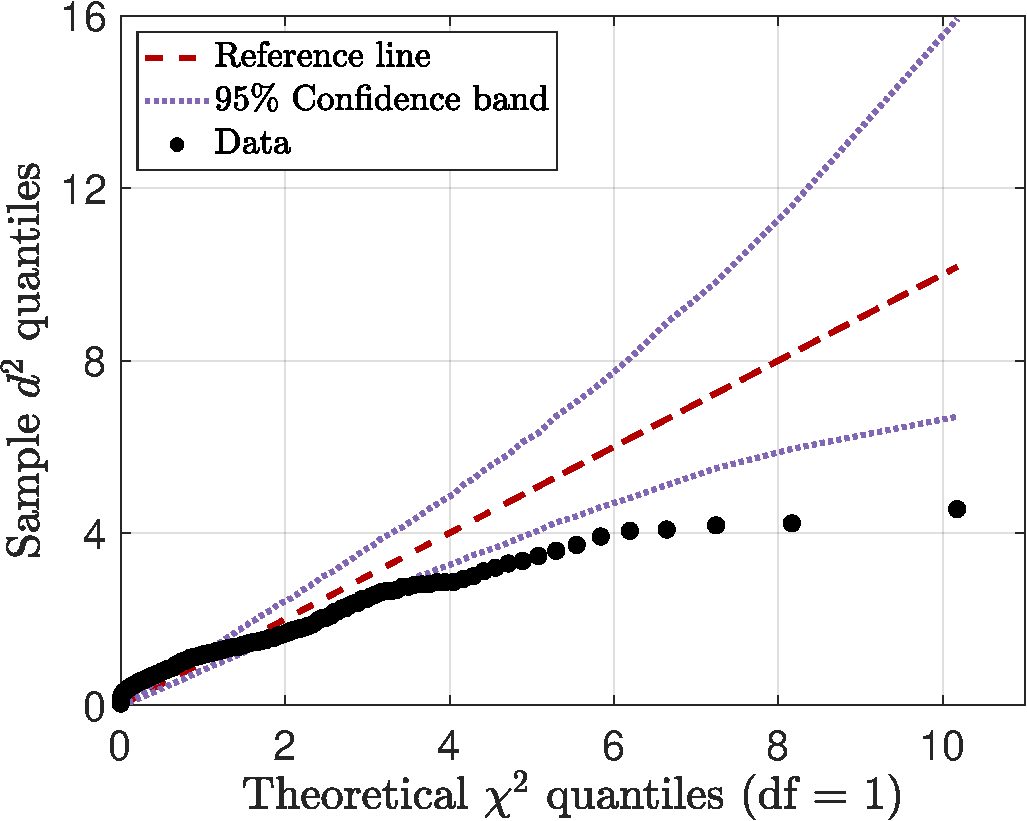
\includegraphics[height=0.36\linewidth]{./figures/test_normal.pdf}&
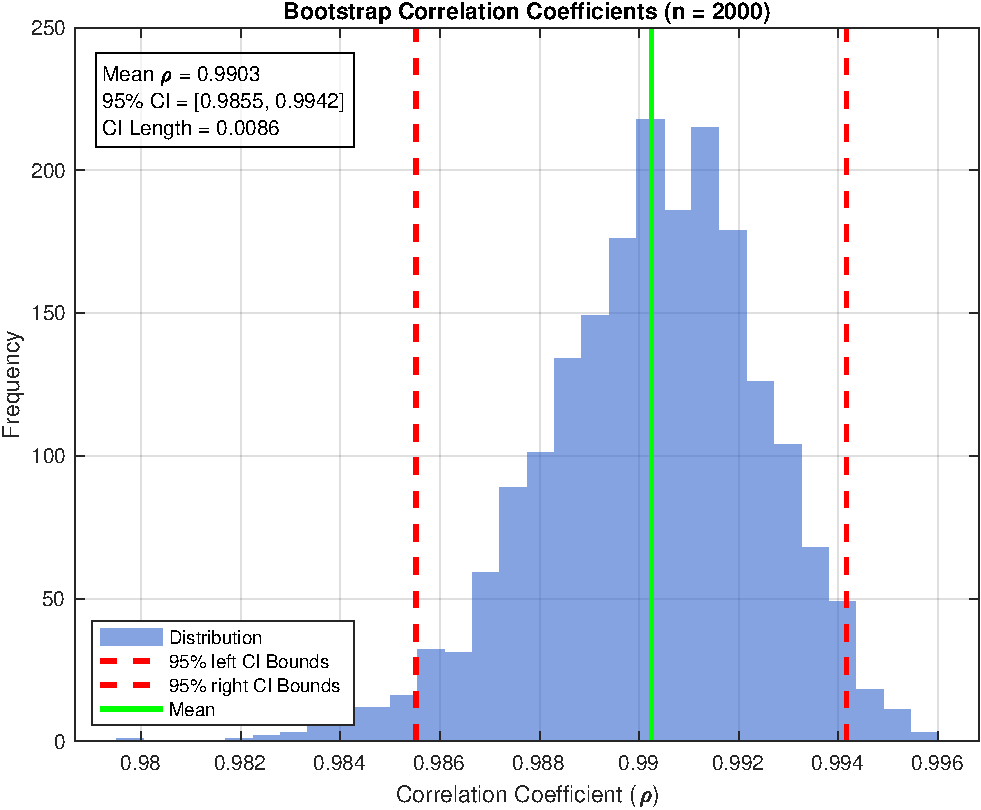
\includegraphics[height=0.36\linewidth]{./figures/CI_bootstrap.pdf}
\end{tabular}
\caption{Left: quantile-quantile plot of sample $d^2$ quantiles v.s. theoretical $\chi^2$ quantiles. The figure is generated with 400 samples of direct solver on the reference mesh. 95\% confidence interval generated with Bootstrap with 400 samples with 1000 repeated sampling. The normal distribution is plotted with the reference red line. Right: 95\% confidence interval generated with Bootstrap.}
\label{fig:Test_normal}
\end{figure}
%
% Figure \ref{fig:Test_normal} shows that $u_{h,1}(\cdot, \boldsymbol{\omega})$ is not normal. If it is Gaussian, $d^2$ should follow $\chi^2$ distribution and we should expect the data to be around the reference line of normal distribution and its associated confidence interval. However, the squared distance of each data deviate from the red line. The sample quatiles has downward inflection, which indidates that the data is left skewed.

% If at least $u_{h,1}(\cdot, \boldsymbol{\omega})$ and $u_{h,k}(\cdot, \boldsymbol{\omega})$ are not normal, $u_{h,1}(\cdot, \boldsymbol{\omega})$ and $u_{h,k}(\cdot, \boldsymbol{\omega})$ are not bivariate normal, therefore, they are not bivariate normal.


We adopt a dynamic strategy, outlined in Algorithm~\ref{algo:Parameter_Estimation}, that iteratively refines sample statistics. To ensure unbiased and statistically independent estimates, each pairwise correlation coefficient $\rho_{1,k}$ between the high-fidelity model and the $k$-th low-fidelity model is computed using independently drawn sample sets. Consequently, for $K$ low-fidelity models and $Q$ pilot samples per correlation, the total number of high-fidelity evaluations is $KQ$. In our experiments, we assume a correlation estimation error of $\delta_1 = 10\%$ and use an error-splitting parameter $\theta_1 = 0.5$. $z_{\alpha/2} = 1.96$ ($95\%$ confidence interval. The corresponding parameter estimation costs and pilot sample sizes -- computed via Algorithm~\ref{algo:Parameter_Estimation} -- are given in Table~\ref{Tab:Offline_cost} for each spatial level $L$.



Table~\ref{Tab:MFMC_parameters} reports the estimated correlation coefficients for all candidate low-fidelity models prior to model selection under the dynamic strategy. For comparison, the table also includes benchmark values obtained using a fixed sample size of 500. The resulting sampling cost efficiencies $\xi$, computed using \eqref{eq:MFMC_sampling_cost_efficiency}, are
%
\begin{alignat*}{2}
    &\text{Fixed-sample:}\quad &\xi = 8.85\times 10^{-3}, 2.76\times 10^{-3}, 7.70\times 10^{-4}, 5.93\times 10^{-4},\\
    &\text{Dynamic:}\quad &\xi =8.81\times 10^{-3}, 2.65\times 10^{-3}, 7.22\times 10^{-4},  5.97\times 10^{-4}.
\end{alignat*}
%
for spatial levels $L=2,3,4,5$, respectively. These values differ by less than 5\%.
Furthermore, we compute the constant $A$ in \eqref{eq:delta_xi_bound} for each high-fidelity model at $L=2,3,4,5$, obtaining values of 2.69, 2.68, 2.53, and 2.22, respectively. Notably, the theoretical upper bound in \eqref{eq:delta_xi_bound} significantly overestimates the actual variation in $\xi$, indicating that small deviations in parameter estimates have minimal impact on overall efficiency. A comparison of correlation coefficients between the dynamic sampling and fixed sample size approach further supports this conclusion, as the two methods yield highly consistent results, differing by at most two decimal places in most cases. These findings demonstrate the effectiveness of dynamic sampling in achieving accurate parameter estimation while reducing computational costs.







%
\begin{table}[ht]
\centering
\scalebox{0.8}{
\begin{tabular}{|c|c|c|c|c|c|c|c|c|c|c|c|c|c|c|c|c|c|c|}
\hline
\multicolumn{8}{|c|}{Dynamic sampling} \\
\cline{1-8}	
\multirow{2}{*}{$\epsilon$}&\multicolumn{1}{|c|}{$\ell$} &0&1&2&3&4&5\\
\cline{2-8}	
&\multicolumn{1}{|c|}{$M_\ell$} &$2685$ &$8019$ &$30449$ &$120697$ &$484080$ &$1934365$\\
\hline
\multirow{1}{*}{$6\times 10^{-3}\;\;\sim \;\;8\times 10^{-3}$} 
&\multicolumn{1}{|c|}{$\rho_{1,k} (k=3-\ell)$}&9.7892e-01&9.9751e-01&1&\multicolumn{3}{c|}{}\\
% &\multicolumn{1}{|c|}{Candidate model $k$} &$\widehat u_{h,3}$&$\widehat u_{h,2}$&$\widehat u_{h,1}$&\multirow{3}{*}{}&\multirow{3}{*}{}&\multirow{3}{*}{}\\
\cline{2-5}		
% &\multicolumn{1}{|c|}{$\sigma_{k}$}&9.7398e-03  &1.2180e-02 &1.1058e-02&&&\\
% \cline{2-5}	
% &\multicolumn{1}{|c|}{$\text{Cov}\left(\widehat u_{h,1},\widehat u_{h,k}\right)$}&1.0368e-04&1.3773e-04 &-&&&\\
% \cline{2-5}
% \hline
% &\multicolumn{1}{|c|}{Sample no. and time}&50&1.6612e+02\\
% \hline
% &\multicolumn{1}{|c|}{$\xi$}&8.81e-03\\
\hline
\multirow{1}{*}{$2\times 10^{-3}\;\;\sim \;\;4\times 10^{-3}$} 
&\multicolumn{1}{|c|}{$\rho_{1,k} (k=4-\ell)$}&9.8352e-01&9.9660e-01 &9.9938e-01&1&&\\
\cline{2-6}	
% &\multicolumn{1}{|c|}{Candidate model $k$} &$\widehat u_{h,4}$&$\widehat u_{h,3}$&$\widehat u_{h,2}$&$\widehat u_{h,1}$&\multirow{3}{*}{}&\multirow{3}{*}{}\\
% \cline{2-6}		
% &\multicolumn{1}{|c|}{$\sigma_{k}$}&9.5275e-03&1.2174e-02&9.1390e-03&1.0404e-02&&\\
% \cline{2-6}	
% &\multicolumn{1}{|c|}{$\text{Cov}\left(\widehat u_{h,1},\widehat u_{h,k}\right)$} &1.0227e-04&1.3680e-04 &8.2654e-05&- &&\\

% \hline
% &\multicolumn{1}{|c|}{Sample no. and time}&30&4.5414e+02\\
% \hline
% &\multicolumn{1}{|c|}{$\xi$}&2.65e-03\\
\hline
% \multirow{2}{*}{$4\times 10^{-4}\;\;\sim \;\;1\times 10^{-3}$} &\multicolumn{1}{|c|}{Candidate model $k$} &$\widehat u_{h,5}$&$\widehat u_{h,4}$&$\widehat u_{h,3}$&$\widehat u_{h,2}$&$\widehat u_{h,1}$&\multirow{3}{*}{}\\
%  \cline{2-7}	
% &\multicolumn{1}{|c|}{$\sigma_{k}$}&9.7260e-03&1.2496e-02&1.2300e-02&1.1717e-02&1.1606e-02  &\\
% \cline{2-7}	
% &\multicolumn{1}{|c|}{$\text{Cov}\left(\widehat u_{h,1},\widehat u_{h,k}\right)$}&1.0487e-04&1.4379e-04&1.4983e-04&1.3733e-04  &- &\\
\cline{2-7}	
\multirow{1}{*}{$4\times 10^{-4}\;\;\sim \;\;1\times 10^{-3}$}&\multicolumn{1}{|c|}{$\rho_{1,k} (k=5-\ell)$}&9.8288e-01&9.9682e-01&9.9941e-01  &9.9976e-01&1 &\\
% \hline
% &\multicolumn{1}{|c|}{Sample no. and time}&50&3.8655e+03\\
% \hline
% &\multicolumn{1}{|c|}{$\xi$}&7.22e-04\\
\hline
% \multirow{2}{*}{$2\times 10^{-4}$} &\multicolumn{1}{|c|}{Candidate model $k$} &$\widehat u_{h,6}$&$\widehat u_{h,5}$&$\widehat u_{h,4}$&$\widehat u_{h,3}$&$\widehat u_{h,2}$&$\widehat u_{h,1}$\\
% \cline{2-8}
% &\multicolumn{1}{|c|}{$\sigma_{k}$}&9.3878e-03&1.0134e-02&1.3305e-02&9.4344e-03&9.7624e-03&1.0524e-02\\
% \cline{2-8}	
% &\multicolumn{1}{|c|}{$\text{Cov}\left(\widehat u_{h,1},\widehat u_{h,k}\right)$}&1.0164e-04&1.0662e-04&1.1679e-04&1.1589e-04&1.0646e-04&-\\
\cline{2-8}	
\multirow{1}{*}{$2\times 10^{-4}$}&\multicolumn{1}{|c|}{$\rho_{1,k} (k=6-\ell)$}&9.8044e-01&9.9787e-01&9.9960e-01&9.9975e-01&9.9970e-01   &1\\
% \hline
% &\multicolumn{1}{|c|}{Sample no. and time}&30&1.2147e+04\\
% \hline
% &\multicolumn{1}{|c|}{$\xi$}&5.97e-04\\
\hline
\multicolumn{8}{|c|}{Benchmark samping with 500 samples} \\
\hline
% \multirow{2}{*}{$6\times 10^{-3}\;\;\sim \;\;8\times 10^{-3}$} &\multicolumn{1}{|c|}{Candidate model $k$} &$\widehat u_{h,3}$&$\widehat u_{h,2}$&$\widehat u_{h,1}$&\multirow{3}{*}{}&\multirow{3}{*}{}&\multirow{3}{*}{}\\
% \cline{2-5}		
% &\multicolumn{1}{|c|}{$\sigma_{k}$}&9.5720e-03   &1.1549e-02   &1.0939e-02&&&\\
% \cline{2-5}	
% &\multicolumn{1}{|c|}{$\text{Cov}\left(\widehat u_{h,1},\widehat u_{h,k}\right)$}&1.0286e-04&1.2604e-04&-&&&\\
% \cline{2-5}
\multirow{1}{*}{$6\times 10^{-3}\;\;\sim \;\;8\times 10^{-3}$}&\multicolumn{1}{|c|}{$\rho_{1,k} (k=3-\ell)$}&9.8238e-01&9.9762e-01&1&&&\\
% \hline
% &\multicolumn{1}{|c|}{$\xi$}&8.8504e-03\\
\hline
% \multirow{2}{*}{$2\times 10^{-3}\;\;\sim \;\;4\times 10^{-3}$} &\multicolumn{1}{|c|}{Candidate model $k$} &$\widehat u_{h,4}$&$\widehat u_{h,3}$&$\widehat u_{h,2}$&$\widehat u_{h,1}$&\multirow{3}{*}{}&\multirow{3}{*}{}\\
% \cline{2-6}	
% &\multicolumn{1}{|c|}{$\sigma_{k}$}&9.5720e-03   &1.1549e-02   &1.1001e-02   &1.0836e-02 &&\\
% \cline{2-6}	
% &\multicolumn{1}{|c|}{$\text{Cov}\left(\widehat u_{h,1},\widehat u_{h,k}\right)$} &1.0206e-04 &1.2480e-04 &1.1911e-04 &- &&\\
% \cline{2-6}	
\multirow{1}{*}{$2\times 10^{-3}\;\;\sim \;\;4\times 10^{-3}$}&\multicolumn{1}{|c|}{$\rho_{1,k} (k=4-\ell)$}&9.8394e-01&9.9720e-01 &9.9919e-01&1&&\\
% \hline
% &\multicolumn{1}{|c|}{$\xi$}&2.7609e-03\\
\hline
% \multirow{2}{*}{$4\times 10^{-4}\;\;\sim \;\;1\times 10^{-3}$} &\multicolumn{1}{|c|}{Candidate model $k$} &$\widehat u_{h,5}$&$\widehat u_{h,4}$&$\widehat u_{h,3}$&$\widehat u_{h,2}$&$\widehat u_{h,1}$&\multirow{3}{*}{}\\
%  \cline{2-7}	
% &\multicolumn{1}{|c|}{$\sigma_{k}$}&9.5720e-03   &1.1549e-02   &1.1001e-02   &1.0838e-02   &1.0840e-02  &\\
% \cline{2-7}	
% &\multicolumn{1}{|c|}{$\text{Cov}\left(\widehat u_{h,1},\widehat u_{h,k}\right)$}&1.0209e-04 &1.2485e-04 &1.1916e-04 &1.1745e-04 &- &\\
% \cline{2-7}	
\multirow{1}{*}{$4\times 10^{-4}\;\;\sim \;\;1\times 10^{-3}$} &\multicolumn{1}{|c|}{$\rho_{1,k} (k=5-\ell)$}&9.8392e-01 &9.9727e-01 &9.9925e-01 &9.9977e-01 &1 &\\
% \hline
% &\multicolumn{1}{|c|}{$\xi$}&7.7012e-04\\
\hline
% \multirow{2}{*}{$2\times 10^{-4}$} &\multicolumn{1}{|c|}{Candidate model $k$} &$\widehat u_{h,6}$&$\widehat u_{h,5}$&$\widehat u_{h,4}$&$\widehat u_{h,3}$&$\widehat u_{h,2}$&$\widehat u_{h,1}$\\
% \cline{2-8}
% &\multicolumn{1}{|c|}{$\sigma_{k}$}&9.5720e-03   &1.1549e-02   &1.1001e-02   &1.0838e-02   &1.0812e-02  &1.0840e-02\\
% \cline{2-8}	
% &\multicolumn{1}{|c|}{$\text{Cov}\left(\widehat u_{h,1},\widehat u_{h,k}\right)$}&1.0209e-04&1.2485e-04&1.1916e-04&1.1745e-04&1.1717e-04&-\\
% \cline{2-8}	
\multirow{1}{*}{$2\times 10^{-4}$}&\multicolumn{1}{|c|}{$\rho_{1,k} (k=6-\ell)$}&9.8390e-01   &9.9728e-01   &9.9925e-01   &9.9977e-01   &9.9976e-01   &1\\
% \hline
% &\multicolumn{1}{|c|}{$\xi$}&5.9298e-04\\
\hline
\end{tabular}}
\caption{Estimated statistical parameters for different tolerances $\epsilon$ in terms of nMSE. The top section presents results from the dynamic strategy with $\delta=10\%, \theta_1=0.5$, while the bottom section corresponds to 500 pilot samples. The high-fidelity model $\widehat u_{h,1}$ is the finite element solution on spatial grid level $L$, with $\rho_{1,1}=1$ for all entries in the table. Candidate low-fidelity models $\widehat u_{h,k}$ ($k \geq 2$) are generated using 25 sparse grid nodes (level $q=1$) on spatial grids of levels 0 to $L-1$. All parameters are estimated using Welford's algorithm.}
\label{Tab:MFMC_parameters}
\end{table}
%






% %
% \begin{table}[ht]
% \centering
% \scalebox{0.8}{
% \begin{tabular}{|c|c|c|c|c|c|c|c|c|c|c|c|c|c|c|c|c|c|c|}
% \cline{1-8}	
% \multirow{2}{*}{$\epsilon$}&\multicolumn{1}{|c|}{$\ell$} &0&1&2&3&4&5\\
% \cline{2-8}	
% &\multicolumn{1}{|c|}{$M_\ell$} &$2685$ &$8019$ &$30449$ &$120697$ &$484080$ &$1934365$\\
% \hline
% \multirow{2}{*}{$6\times 10^{-3}\;\;\sim \;\;8\times 10^{-3}$} &\multicolumn{1}{|c|}{Candidate model $k$} &$\widehat u_{h,3}$&$\widehat u_{h,2}$&$\widehat u_{h,1}$&\multirow{3}{*}{}&\multirow{3}{*}{}&\multirow{3}{*}{}\\
% % \cline{2-5}		
% % &\multicolumn{1}{|c|}{$\sigma_{k}$}&9.5720e-03   &1.1549e-02   &1.0939e-02&&&\\
% % \cline{2-5}	
% % &\multicolumn{1}{|c|}{$\text{Cov}\left(\widehat u_{h,1},\widehat u_{h,k}\right)$}&1.0286e-04&1.2604e-04&-&&&\\
% \cline{2-5}
% &\multicolumn{1}{|c|}{$\rho_{1,k}$}&9.8238e-01&9.9762e-01&-&&&\\
% % \hline
% % &\multicolumn{1}{|c|}{$\xi$}&8.8504e-03\\
% \hline
% \multirow{2}{*}{$2\times 10^{-3}\;\;\sim \;\;4\times 10^{-3}$} &\multicolumn{1}{|c|}{Candidate model $k$} &$\widehat u_{h,4}$&$\widehat u_{h,3}$&$\widehat u_{h,2}$&$\widehat u_{h,1}$&\multirow{3}{*}{}&\multirow{3}{*}{}\\
% % \cline{2-6}	
% % &\multicolumn{1}{|c|}{$\sigma_{k}$}&9.5720e-03   &1.1549e-02   &1.1001e-02   &1.0836e-02 &&\\
% % \cline{2-6}	
% % &\multicolumn{1}{|c|}{$\text{Cov}\left(\widehat u_{h,1},\widehat u_{h,k}\right)$} &1.0206e-04 &1.2480e-04 &1.1911e-04 &- &&\\
% \cline{2-6}	
% &\multicolumn{1}{|c|}{$\rho_{1,k}$}&9.8394e-01&9.9720e-01 &9.9919e-01&-&&\\
% % \hline
% % &\multicolumn{1}{|c|}{$\xi$}&2.7609e-03\\
% \hline
% \multirow{2}{*}{$4\times 10^{-4}\;\;\sim \;\;1\times 10^{-3}$} &\multicolumn{1}{|c|}{Candidate model $k$} &$\widehat u_{h,5}$&$\widehat u_{h,4}$&$\widehat u_{h,3}$&$\widehat u_{h,2}$&$\widehat u_{h,1}$&\multirow{3}{*}{}\\
% %  \cline{2-7}	
% % &\multicolumn{1}{|c|}{$\sigma_{k}$}&9.5720e-03   &1.1549e-02   &1.1001e-02   &1.0838e-02   &1.0840e-02  &\\
% % \cline{2-7}	
% % &\multicolumn{1}{|c|}{$\text{Cov}\left(\widehat u_{h,1},\widehat u_{h,k}\right)$}&1.0209e-04 &1.2485e-04 &1.1916e-04 &1.1745e-04 &- &\\
% \cline{2-7}	
% &\multicolumn{1}{|c|}{$\rho_{1,k}$}&9.8392e-01 &9.9727e-01 &9.9925e-01 &9.9977e-01 &- &\\
% % \hline
% % &\multicolumn{1}{|c|}{$\xi$}&7.7012e-04\\
% \hline
% \multirow{2}{*}{$2\times 10^{-4}$} &\multicolumn{1}{|c|}{Candidate model $k$} &$\widehat u_{h,6}$&$\widehat u_{h,5}$&$\widehat u_{h,4}$&$\widehat u_{h,3}$&$\widehat u_{h,2}$&$\widehat u_{h,1}$\\
% % \cline{2-8}
% % &\multicolumn{1}{|c|}{$\sigma_{k}$}&9.5720e-03   &1.1549e-02   &1.1001e-02   &1.0838e-02   &1.0812e-02  &1.0840e-02\\
% % \cline{2-8}	
% % &\multicolumn{1}{|c|}{$\text{Cov}\left(\widehat u_{h,1},\widehat u_{h,k}\right)$}&1.0209e-04&1.2485e-04&1.1916e-04&1.1745e-04&1.1717e-04&-\\
% \cline{2-8}	
% &\multicolumn{1}{|c|}{$\rho_{1,k}$}&9.8390e-01   &9.9728e-01   &9.9925e-01   &9.9977e-01   &9.9976e-01   &-\\
% % \hline
% % &\multicolumn{1}{|c|}{$\xi$}&5.9298e-04\\
% \hline
% \end{tabular}}
% \caption{Estimated statistical parameters for various predetermined tolerances $\epsilon$ in terms of nMSE with 500 samples for approximating parameters between each low fidelity models and the corresponding high fidelity model. The high-fidelity model $\widehat u_{h,1}$ represents the finite element solution to the free boundary problem on a spatial grid of level $L$, ensuring the discretization error meets accuracy requirements. Candidate low-fidelity models $\widehat u_{h,k}$ for $k \geq 2$ are generated using 25 sparse grid nodes (with level $q=1$) on spatial grids from levels 0 to $L-1$. All parameters are estimated using Welford's dynamic sampling algorithm with a stopping criterion requiring a relative error of $10^{-4}$ for all parameters.}
% \label{Tab:MFMC_parameters}
% \end{table}
% %

Using the same experimental setup for estimating statistical parameters with a fixed sample size of 500 at a tolerance of $\epsilon=2\times 10^{-4}$ (as reported in Table \ref{Tab:MFMC_parameters}), we compute the per-sample costs for both the high-fidelity model $(W_\ell)$ and low-fidelity models $(W_\ell^e)$ across spatial levels 0 to 5. The results, shown in the left plot of Figure \ref{fig:CostEstimatePlot}, illustrate the expenses incurred at different spatial levels.  Before model selection, the cost per sample $C_k$ in the MFMC framework is linked to the model evaluation cost per sample by $C_1=W_{L}$ for the high-fidelity model and $C_k=W_{L-k+1}^e$ for the low-fidelity models. However, not all candidate low-fidelity models are necessarily included in the final MFMC estimator, as their associated parameters must satisfy the conditions of Theorem \ref{thm:Sample_size_est}. The model selection algorithm filters out low-fidelity models that fail to enhance computational efficiency. For instance, when $\epsilon=2\times 10^{-4}$, the correlation coefficients associated with $\widehat u_{h,2}$ and  $\widehat u_{h,3}$ violate the non-increasing property (Condition (i) of Theorem \ref{thm:Sample_size_est}), leading to the exclusion of $\widehat u_{h,2}$ from the final estimator. 

% %
% \begin{table}[ht]
% \centering
% \scalebox{0.8}{
% \begin{tabular}{c|c|c|c|c|c|c|c|c|c|c|c|c|c|c|c|c|c|c|}
% \cline{1-7}	
% \multicolumn{1}{|c|}{$\ell$} &0&1&2&3&4&5\\
% \hline
% \multicolumn{1}{|c|}{$M_\ell$} &$2685$ &$8019$ &$30449$ &$120697$ &$484080$ &$1934365$\\
% % \hline
% % \multicolumn{1}{|c|}{Model $k$} &$f_1$&$f_2$&$f_3$&$f_4$&$f_5$&$f_6$\\
% \hline
% \multicolumn{1}{|c|}{$W_\ell$ direct solve}&4.88e-02 &1.49e-01 &6.33e-01 &3.23e+00 &1.55e+01 &7.30e+01\\
% \hline
% \multicolumn{1}{|c|}{$W_\ell^e$ surrog evaluation}&2.68e-04   &5.06e-04   &1.40e-03   &7.03e-03   &2.17e-02   &9.71e-02\\
% \hline
% % \multicolumn{1}{|c|}{$C_\ell$ surrog evaluation( nodes)-source term}&\\
% % \hline
% \end{tabular}}
% \caption{The number of spatial grid points $M_\ell$, cost per sample for both direct computation $W_\ell$ and surrogate evaluation $W_\ell^e$ at an increasing spatial grid level $\ell = 0$ to 5.}
% % and surrogate evaluation with level $q=1$ sparse grid nodes ($P=$)  in the source term.}
% \label{Tab:Dof}
% \end{table}
% %

%
\begin{figure}[ht!]\centering
\begin{tabular}{cc}
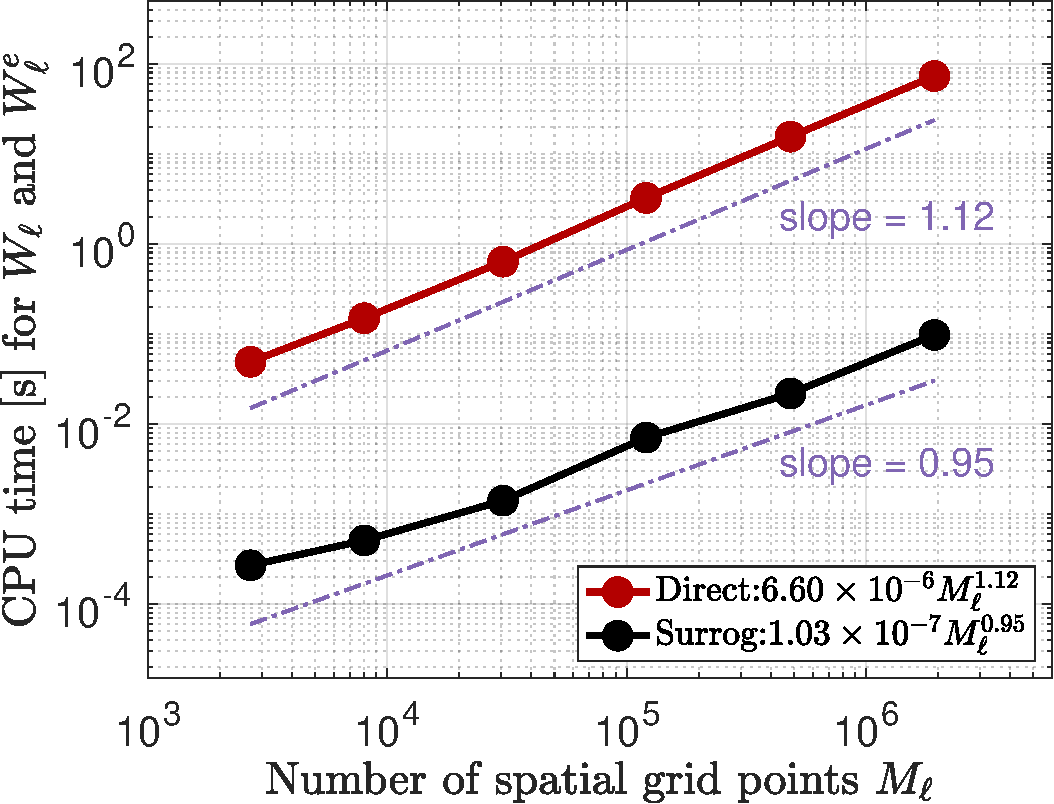
\includegraphics[height=0.36\linewidth]{./figures/CostPerSample_Ml.pdf}&
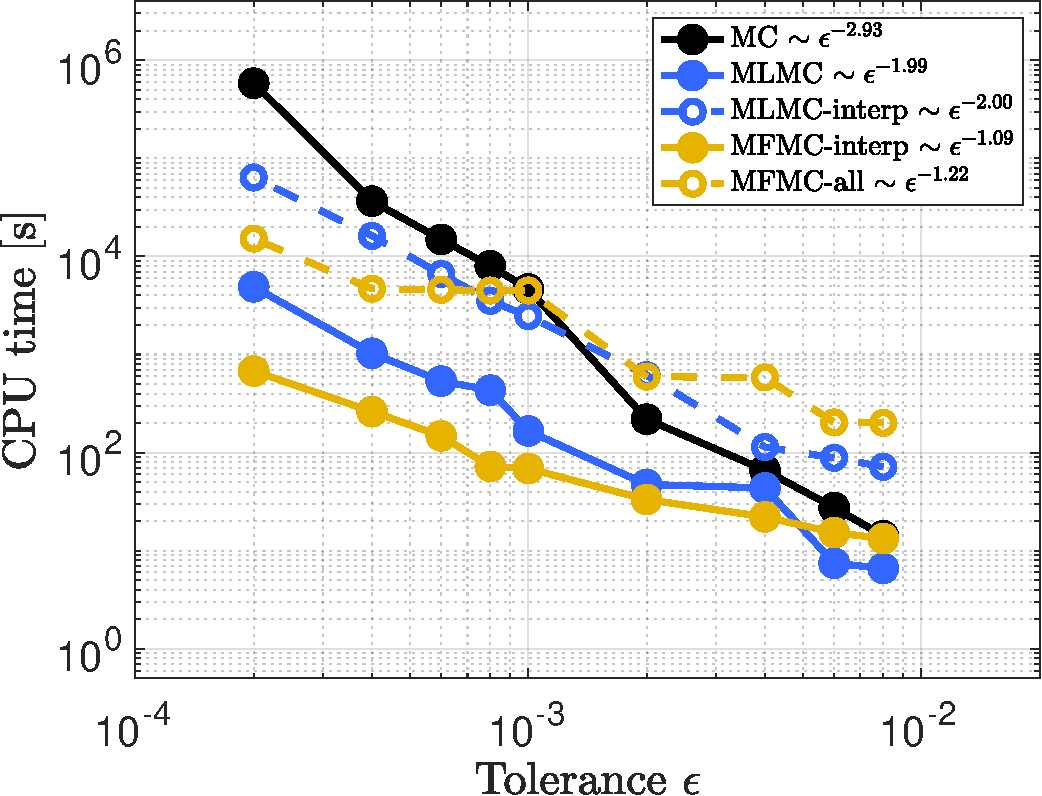
\includegraphics[height=0.36\linewidth]{./figures/Cost_epsilon.pdf}
\end{tabular}
\caption{Left: Mean CPU times of 500 realizations for direct computations $W_\ell$ and surrogate evaluations $W_\ell^e$ versus the number of spatial grid points $M_\ell$ for $\ell = 0$ to 5. Right: Total CPU time versus $\epsilon$ for different simulation methods.}
\label{fig:CostEstimatePlot}
\end{figure}
%




 
 % While the offline preparation incurs non-negligible computational expenses, these costs are justified by the substantial savings achieved during large-scale online sampling, particularly in applications requiring thousands of high-fidelity model evaluations. As a one-time expense, the precomputed surrogates and statistical parameters are reused throughout the online phase, amortizing the initial overhead across all subsequent multi-fidelity Monte Carlo realizations.







% %
% \begin{table}[ht]
% \centering
% \scalebox{0.8}{
% \begin{tabular}{c|c|c|c|c|c|c|c|c|c|c|c|c|c|c|c|c|c|c|}
% \cline{1-7}	
% \multicolumn{1}{|c|}{$\ell$} &0&1&2&3&4&5\\
% \hline
% \multicolumn{1}{|c|}{$M_\ell$} &$2685$ &$8019$ &$30449$ &$120697$ &$484080$ &$1934365$\\
% \hline
% \multicolumn{1}{|c|}{Model $k$} &$\widehat u_{h,5}$&$\widehat u_{h,4}$&$\widehat u_{h,3}$&$\widehat u_{h,2}$&&\\
% \hline
% \multicolumn{1}{|c|}{$\rho_{1,k}$ (24 nodes), ref l=3}&0.9802&0.9958 &0.9976&0.9984&&\\
% \hline
% \multicolumn{1}{|c|}{$\sigma_{k}$}&9.3826e-05 &1.374e-04 &1.2405e-04 &1.2016e-04 &&\\
% \hline
% \multicolumn{1}{|c|}{Covariance} &1.0807e-04 &1.3283e-04 &1.2646e-04 &1.2457e-04 &&\\
% \hline
% \end{tabular}}
% \caption{$\epsilon = 4\times 10^{-3}\;\;\& \;\;2\times 10^{-3}$. High fidelity model: finite element solution on mesh with 120697 grid nodes. $\sigma_1 = 1.2955e-04$. The data are estimated using 500 samples. The selected models are $[\widehat u_{h,2},\widehat u_{h,4},\widehat u_{h,5}]$.}
% % \label{Tab:Dof}
% \end{table}
% %

% %
% \begin{table}[ht]
% \centering
% \scalebox{0.8}{
% \begin{tabular}{c|c|c|c|c|c|c|c|c|c|c|c|c|c|c|c|c|c|c|}
% \cline{1-7}	
% \multicolumn{1}{|c|}{$\ell$} &0&1&2&3&4&5\\
% \hline
% \multicolumn{1}{|c|}{$M_\ell$} &$2685$ &$8019$ &$30449$ &$120697$ &$484080$ &$1934365$\\
% \hline
% \multicolumn{1}{|c|}{Model $k$} &$\widehat u_{h,6}$&$\widehat u_{h,5}$&$\widehat u_{h,4}$&$\widehat u_{h,3}$&$\widehat u_{h,2}$&\\
% \hline
% \multicolumn{1}{|c|}{$\rho_{1,k}$ (24 nodes), ref l=3}&9.0103e-01 &9.2531e-01 &9.2415e-01 &9.2366e-01 &9.2307e-01 &\\
% \hline
% \multicolumn{1}{|c|}{$\sigma_{k}$}&1.1064e-04 &1.3571e-04 &1.2930e-04 &1.2757e-04  &1.2742e-04  &\\
% \hline
% \multicolumn{1}{|c|}{Covariance}&8.9789e-05 &1.2808e-04 &1.1657e-04 &1.1358e-04 &1.1346e-04 &\\
% \hline
% \end{tabular}}
% \caption{$\epsilon = 1\times 10^{-3}\;\;\& \;\;8\times 10^{-4}\;\;\& \;\;6\times 10^{-4}\;\;\& \;\;4\times 10^{-4}$. High fidelity model: finite element solution on mesh with 484080 grid nodes. $\sigma_1 = 1.6794e-04$. The data are estimated using 500 samples.}
% % \label{Tab:Dof}
% \end{table}
% %





% =============================
\subsection{Sampling (online) cost}
% =============================
After the offline procedure, the selected low-fidelity models and estimated statistical parameters, including correlation coefficients
$\rho_{1,k}$ and weights $\alpha_k$, are used to compute the MFMC estimator in the online phase. The unbiasedness of the MFMC estimator relies on the independence of the samples used to estimate $\alpha_k$ from those used in online sampling. This follows from the expectation property $\mathbb{E}(\alpha_k Y_k) = \alpha_k \mathbb{E}(Y_k)$ and the condition $\mathbb{E}(Y_k) = 0$ for $k=2,\ldots, K$. Therefore, maintaining statistical independence between parameter estimation and online sampling is essential to prevent correlations between $\alpha_k$ and $Y_k$, which would otherwise lead to bias in the estimator. However, in practical applications, particularly when high-fidelity model evaluations are computationally expensive, reusing samples for both parameter estimation and online sampling may be necessary. In such cases, the weights $\alpha_k$ become sample-dependent random variables, leading to a correlation between $\alpha_k$  and the correction term $Y_k$. This dependence introduces bias, as the expectation satisfies $\mathbb{E}(\alpha_k Y_k) = \mathbb{E}(\alpha_k Y_k)-\mathbb{E}(\alpha_k)\mathbb{E}(Y_k) = \text{Cov}(\alpha_k,Y_k)\neq 0$, resulting in $\mathbb{E}(A^{\text{MF}})\neq \mathbb{E}(Y_1)$. Prior study \cite{KoFaPeDiJeNeBu:2022} has demonstrated that in certain applications, sample reuse has a negligible effect on the estimator accuracy.  In contrast, MLMC does not suffer from this issue, as it uses fixed weights $\alpha_k =1$, allowing sample reuse for parameter estimation without introducing bias.

The online sampling cost for computing the MFMC estimator is shown in the right plot of Figure \ref{fig:CostEstimatePlot}, where the total cost scales approximately as $\epsilon^{-1.09}$. Table \ref{Tab:MFMC_parameters} provides further insight into this behavior. When $\epsilon=2\times 10^{-4}$, the term $\sqrt{C_1(1-\rho_{1,2}^2)}$ evaluates to 0.191, whereas the summation term $\sum_{k=2}^K\sqrt{C_k(\rho_{1,k}^2-\rho_{1,k+1}^2)}$ is 0.0239. This result indicates that the computational cost of the high-fidelity model significantly outweighs that of all selected low-fidelity models combined. Consequently, in Theorem \ref{thm:Sample_cost_est}, the parameter $c_1$ is much larger than $c_2$,  implying that the dominant cost contribution arises from the high-fidelity model, which scales as $\epsilon^{\frac{\beta-\gamma}{2\alpha}}$. As a result, the MFMC sampling cost $\mathcal{W}^{\text{MF}}$ follows the asymptotic behavior $\epsilon^{-2+\frac{\beta-\gamma}{\alpha}}$. Furthermore, Table \ref{Tab:MFMC_parameters} shows that $\rho_{1,2}\approx 1$ for nearly all values of $\epsilon$, suggesting that the low-fidelity model $\widehat u_{h,2}$ closely resembles the direct nonlinear solve. According to \cite[Lemma 2]{PeGuWi:2018}, the correlation decay between consecutive MFMC models follows $\rho_{1,\ell}^2 - \rho_{1,\ell-1}^2\simeq M_\ell^{-\beta}$, where $\beta$ characterizes the variance decay rate of the MLMC correction term and is estimated as $\beta\approx 2$ in \cite{ElLiSa:2023}. Using parameter estimates from \cite{ElLiSa:2023, ElLiSa:2025}, where $\alpha\approx 1, \beta_1\approx 1.52, \gamma_1=1$, along with the estimate $\gamma\approx 1.1$ from the left plot of Figure \ref{fig:CostEstimatePlot}, we find that the total MFMC sampling cost $\mathcal{W}^{\text{MF}}$ scales as $\epsilon^{-1.09}$, which closely matches the experimental results. For comparison, the Monte Carlo method exhibits a theoretical cost scaling of $\epsilon^{-2-\gamma/\alpha}\simeq \epsilon^{-3.1}$, while the multilevel Monte Carlo method follows $\epsilon^{-2}$. These theoretical predictions align well with the experimentally observed scalings of $\epsilon^{-2.93}$ for Monte Carlo and $\epsilon^{-1.99}$ for MLMC.

The right plot of Figure \ref{fig:CostEstimatePlot} also shows the total online and offline costs of the MFMC approach (yellow dotted curve), where correction terms $Y_k$ in the estimator \eqref{eq:MFMC_estimator_Correction} are accumulated after interpolation to a fine common grid. This interpolation reduces extrapolation errors that arise when accumulating sample corrections on a non-nested, geometry-conforming mesh. The blue dotted line represents the MLMC method, which similarly applies interpolation to a fine common grid. For larger values of $\epsilon$ (above $10^{-3}$), MFMC with combined costs incurs higher costs than both MC and MLMC with interpolation due to the additional expense of estimating statistical parameters. However, as $\epsilon$ decreases, MFMC becomes more efficient and eventually outperforms both MC and MLMC with interpolation. Table \ref{Tab:CPU_time} presents the relative speedup of different methods using MC as a baseline. While speedup is inversely related to cost efficiency, it deviates from the theoretical cost efficiency computed using \eqref{eq:MFMC_sampling_cost_efficiency} due to interpolation cost and other computational overhead.

%
\begin{table}[ht]
	\centering
			\scalebox{0.62}{
   \begin{tabular}{c|c|c|c|c|c|c|c|c|c|c|c|c|}
			\hline
			\multicolumn{1}{|c|}{ }&MC-FE &MLMC-FE&MLMC-FE(Interp)
            % &MFMC-FE 
            &MFMC-FE(Interp)&MFMC-FE(Interp)+upfront\\
			\multicolumn{1}{|c|}{$\epsilon$}&Time &\begin{tabular}{cc} \,\,\,\,\,Time & \,\,\,Speedup \end{tabular}&\begin{tabular}{cc} \,\,\,\,Time & \,\,\,Speedup \end{tabular} &\begin{tabular}{cc} \,\,\,\,Time & \,\,\,Speedup \end{tabular} &\begin{tabular}{cc} \,\,\,\,Time & \,\,\,Speedup \end{tabular}\\
            % &\begin{tabular}{cc} \,\,\,\,Time & \,\,\,Speedup \end{tabular}\\
			\hline
			\multicolumn{1}{|c|}{$8\times 10^{-3} $}&1.42e+01&\begin{tabular}{cc}6.61e+00\,\,\, & 2.1 \end{tabular}&\begin{tabular}{cc}7.17e+01\,\,  &0.2\end{tabular}
            % &\begin{tabular}{cc}7.2998e+00\,\,  &1.9453e+00 \end{tabular} 
            &\begin{tabular}{cc}1.33e+01\,\,   &1.1 \end{tabular} &\begin{tabular}{cc}2.01e+02\,\,  &0.07\end{tabular}\\
			\multicolumn{1}{|c|}{$6\times 10^{-3} $}&2.75e+01&\begin{tabular}{cc}7.44e+00\,\,\, & 3.7 \end{tabular}&\begin{tabular}{cc}8.84e+01\,\,  &0.3\end{tabular}
            % &\begin{tabular}{cc}9.3266e+00\,\, &2.9486e+00 \end{tabular}
            &\begin{tabular}{cc}1.53e+01&1.8
            \end{tabular}&\begin{tabular}{cc}2.03e+02\,\,  &0.1\end{tabular}\\
			\multicolumn{1}{|c|}{$4\times 10^{-3} $}&6.60e+01&\begin{tabular}{cc}4.36e+01\,\,\, & 1.5 \end{tabular}&\begin{tabular}{cc}1.14e+02\,\,  &0.6\end{tabular}
            % &\begin{tabular}{cc}1.9119e+01&3.4521e+00\end{tabular}
            &\begin{tabular}{cc}2.21e+01&3.0
            \end{tabular}&\begin{tabular}{cc}5.84e+02\,\,  &0.1\end{tabular}\\
			\multicolumn{1}{|c|}{$2\times 10^{-3} $}&2.19e+02&\begin{tabular}{cc}4.73e+01\,\, & 4.6\end{tabular}&\begin{tabular}{cc}6.16e+02\,\,  &0.4\end{tabular}
            % &\begin{tabular}{cc}3.0242e+01& 7.2416e+00\end{tabular}
            &\begin{tabular}{cc}3.32e+01&6.6 \end{tabular}&\begin{tabular}{cc}5.95e+02\,\,  &0.4\end{tabular}\\
			\multicolumn{1}{|c|}{$10^{-3} $}&4.66e+03&\begin{tabular}{cr}1.66e+02\,\, & 28.1 \end{tabular}&\begin{tabular}{cc}2.46e+03\,\,  &1.9\end{tabular}
            % &\begin{tabular}{cc}6.5732e+01&7.0894e+01\end{tabular}
            &\begin{tabular}{cc}6.87e+01&67.9
            \end{tabular}&\begin{tabular}{cc}4.49e+03\,\,  &1.0\end{tabular}\\
			\multicolumn{1}{|c|}{$8\times 10^{-4} $}&8.02e+03&\begin{tabular}{cc}4.33e+02\,\, & 18.5 \end{tabular}&\begin{tabular}{cc}3.53e+03\,\,  &2.3\end{tabular}
            % &\begin{tabular}{cc}6.9345e+01&1.1565e+02\end{tabular}
            &\begin{tabular}{cc}7.23e+01&111.0
            \end{tabular}&\begin{tabular}{cc}4.49e+03\,\,  &1.8\end{tabular}\\
			\multicolumn{1}{|c|}{$6\times 10^{-4} $}&1.49e+04&\begin{tabular}{cc}5.36e+02\,\, & 27.8 \end{tabular}&\begin{tabular}{cc}6.63e+03\,\,  &2.2\end{tabular}
            % &\begin{tabular}{cc}1.4482e+02&1.0289e+02\end{tabular}
            &\begin{tabular}{cc}1.48e+02&100.6
            \end{tabular}&\begin{tabular}{cc}4.57e+03\,\,  &3.3\end{tabular}\\
                \multicolumn{1}{|c|}{$4\times 10^{-4} $}&3.66e+04&\begin{tabular}{cc}1.03e+03\,\, & 35.4 \end{tabular}&\begin{tabular}{cc}1.62e+04\,\,  &2.3\end{tabular} &\begin{tabular}{cc}2.62e+02&139.7 \end{tabular}
                % &\begin{tabular}{cc}2.6595e+02&1.3762e+02\end{tabular}
            &\begin{tabular}{cc}4.68e+03\,\,  &7.8\end{tabular}\\
                \multicolumn{1}{|c|}{$2\times 10^{-4} $}&5.84e+05$^{\ast}$\!\!\!&\begin{tabular}{cc}4.90e+03 &119.2 \end{tabular} &\begin{tabular}{cc}6.38e+04\,\,  &9.2\end{tabular}
                % &\begin{tabular}{cc} 6.6985e+02&8.7184e+02 \end{tabular}
                &\begin{tabular}{cc}6.78e+02 &861.2 \end{tabular}&\begin{tabular}{cc}1.52e+04\,\,  &38.4\end{tabular}\\
			\hline
	\end{tabular}
 }
	\caption{CPU time (in seconds) for various simulation methods: Monte Carlo with finite elements (MC-FE), multilevel Monte Carlo with finite elements (MLMC-FE), MLMC-FE with interpolation to a common grid at level $\ell=5$, multifidelity Monte Carlo with finite elements (MFMC-FE) with interpolation to a common grid at level $\ell=5$, and MFMC-FE with interpolation and offline cost inclusion. The table also presents speedup factors for these methods relative to MC-FE at different tolerances $\epsilon$. The CPU time for MC-FE at $\epsilon = 2\times 10^{-4}$ (marked with an asterisk) is an estimate due to prohibitive computational cost.}
	\label{Tab:CPU_time}
\end{table}
%







The efficiency of MFMC relative to MC and MLMC, as observed in Figure \ref{fig:CostEstimatePlot} and Table \ref{Tab:CPU_time}, is closely tied to the distribution of sample sizes across fidelity levels. Table \ref{Tab:SampleSize} provides a detailed breakdown of sample allocation. All methods require a minimum of two samples per level and model. As $\epsilon$ decreases, both discretization and statistical errors are reduced, requiring finer meshes and larger sample sizes across all methods. Compared to MC, MLMC and MFMC shift more samples to low-fidelity models, with MFMC requiring substantially more low-fidelity samples than MLMC. While this increases the total sample count, it ultimately enhances efficiency.




%
\begin{table}[ht]
	\centering
			\scalebox{0.62}{
   \begin{tabular}{c|c|c|c|c|c|c|c|c|c|c|c|c|}
	    \cline{2-7}	
		&\multicolumn{6}{|c|}{ Level $\ell$}\\
			\hline
			\multicolumn{1}{|c|}{$\epsilon$}&0&1&2&3&4&5\\
			\hline
			\multicolumn{1}{|c|}{$8\times 10^{-3} $}&&&5&&&\\
			\multicolumn{1}{|c|}{$6\times 10^{-3} $}&&&9&&&\\
			\multicolumn{1}{|c|}{$4\times 10^{-3} $}&&&&21&&\\
			\multicolumn{1}{|c|}{$2\times 10^{-3} $}&&&&73&&\\
			\multicolumn{1}{|c|}{$10^{-3} $}&&&&&287&\\
			\multicolumn{1}{|c|}{$8\times 10^{-4} $}&&&&&445&\\
			\multicolumn{1}{|c|}{$6\times 10^{-4} $}&&&&&845&\\
                \multicolumn{1}{|c|}{$4\times 10^{-4} $}&&&&&2000&\\
                \multicolumn{1}{|c|}{$2\times 10^{-4} $}&&&&&& 8000$^{\ast}$\!\!\\
			\hline
	\end{tabular}
 \qquad
		\begin{tabular}{c|c|c|c|c|c|c|c|c|c|c|c|c|}
	    \cline{2-7}	
		&\multicolumn{6}{|c|}{ Level $\ell$}\\
			\hline
			\multicolumn{1}{|c|}{$\epsilon$}&0&1&2&3&4&5\\
			\hline
			\multicolumn{1}{|c|}{$8\times 10^{-3} $}&10     &2     &2&&&\\
			\multicolumn{1}{|c|}{$6\times 10^{-3} $}&12     &2     &2&&&\\
			\multicolumn{1}{|c|}{$4\times 10^{-3} $}&22     &5     &2     &2&&\\
			\multicolumn{1}{|c|}{$2\times 10^{-3} $}&163    &26     &5     &2&&\\
			\multicolumn{1}{|c|}{$10^{-3} $}&577   &90    &15     &3     &2&\\
			\multicolumn{1}{|c|}{$8\times 10^{-4} $}&1036 &157 &26 &5 &2&\\
			\multicolumn{1}{|c|}{$6\times 10^{-4} $}&1744 &266 &44 &9 &2&\\
                \multicolumn{1}{|c|}{$4\times 10^{-4} $}&3911 &553 &86 &17 &4&\\
                \multicolumn{1}{|c|}{$2\times 10^{-4} $}&15619 &2298 &370 &57 &12 &2\\
			\hline
	\end{tabular}
 \qquad
		\begin{tabular}{c|c|c|c|c|c|c|c|c|c|c|c|c|c|c|c|c|c|}
	    \cline{2-7}	
		&\multicolumn{6}{|c|}{ Level $\ell$}\\
			\hline
			\multicolumn{1}{|c|}{$\epsilon$}&0&1&2&3&4&5\\
			\hline
			\multicolumn{1}{|c|}{$8\times 10^{-3} $}&24&4&2&&&\\
			\multicolumn{1}{|c|}{$6\times 10^{-3} $}&43&7&2&&&\\
			\multicolumn{1}{|c|}{$4\times 10^{-3} $}&95&12&4&2&&\\
			\multicolumn{1}{|c|}{$2\times 10^{-3} $}&380&46&13&2&&\\
			\multicolumn{1}{|c|}{$10^{-3} $}&2444&301&79&13&2&\\
			\multicolumn{1}{|c|}{$8\times 10^{-4} $}&3819&470&123&21&2&\\
                \multicolumn{1}{|c|}{$6\times 10^{-4} $}&6788&835&218&36&2&\\
			\multicolumn{1}{|c|}{$4\times 10^{-4} $}&15273&1879&489&81&2&\\
                \multicolumn{1}{|c|}{$2\times 10^{-4} $}&97028&13374&2544&335&-&5\\
			\hline
	\end{tabular}
 
 }
	\caption{Optimal sample size estimation for MC-FE (left), MLMC-FE (middle), and MFMC-FE (right) for various tolerance values $\epsilon$. The computational cost for Monte Carlo with a tolerance of $\epsilon = 2\times 10^{-4}$ was prohibitive; therefore, the entry for this tolerance (marked with an asterisk) is an estimate.}
	\label{Tab:SampleSize}
\end{table}
%




% \JLcolor{According to \cite{PeGuWi:2018}, pages A3174 and A3181–A3182, perturbations in the sample variance and sample correlation coefficients have a small impact on the overall sample size and computational work. However, from my perspective, inaccurate estimation of these statistical parameters can also affect the model selection process. If these statistics are not reliably computed, low-fidelity models with misleading characteristics may be selected or rejected incorrectly, potentially undermining the efficiency and accuracy of the MFMC framework. In particular, models that exhibit inconsistent statistical properties violating the two conditions in Theorem \ref{thm:Sample_size_est} could be included, leading to suboptimal model choices for the low-fidelity approximations and, consequently, affecting the overall performance of the multi-fidelity estimator.}






% =============================
\subsection{Properties of plasma boundary and geometric descriptors}
% =============================
As shown in \cite{ElLiSa:2023}, multilevel Monte Carlo faces challenges when handling plasma boundary distortions caused by extrapolation errors during cross-level sample correction on non-nested, geometry-conforming meshes. These errors result from spatial resolution mismatches when coarse-grid corrections are aggregated across multiple levels. To mitigate this distortion, MLMC solutions are interpolated onto a unified fine grid at level $\ell=5$, ensuring consistency in resolution while preserving the geometric fidelity of the plasma boundary. Similarly, in the multi-fidelity Monte Carlo (MFMC) approach, sample corrections for various low-fidelity models are generated using stochastic collocation on the same geometry-conforming coarse grids. To maintain consistency in spatial resolution, these corrections are projected onto the same common fine mesh. 

Figure \ref{fig:QoI_plot} illustrates the plasma boundary obtained using Monte Carlo, MLMC, and MFMC sampling methods. The MFMC-generated boundary closely resembles the Monte Carlo benchmark,  demonstrating that proper interpolation and projection effectively reduce geometric distortions. Table \ref{Tab:QoI_GeoInfo} further quantifies this agreement, showing that the geometric descriptors of both MLMC with interpolation and MFMC align with the Monte Carlo benchmark to two decimal places. 



%=====================================================================================
% \noindent \textbf{Plasma boundary.} 
%=====================================================================================






% %
% \begin{table}[ht]
% \centering
% \scalebox{0.8}{
% \begin{tabular}{c|c|c|c|c|c|c|c|c|c|c|c|c|c|c|c|c|c|c|}
% \cline{1-7}	
% \multicolumn{1}{|c|}{Dof} &$1934365$&$484080$&$120697$&$30449$&$8019$&$2685$\\
% \hline
% \multicolumn{1}{|c|}{Model $k$} &$f_1$&$f_2$&$f_3$&$f_4$&$f_5$&$f_6$\\
% % \hline
% % \multicolumn{1}{|c|}{$C_k$ direct solve}&1.2029e+02&2.6478e+01&5.3710e+00&1.1269e+00&2.9300e-01&9.6419e-02\\
% % \hline
% % \multicolumn{1}{|c|}{$C_k$ surrog evaluation(24 nodes)}&1.2595e-01&2.9694e-02&9.1085e-03&3.0580e-03&1.1869e-03&2.5127e-04\\
% \hline
% \multicolumn{1}{|c|}{$\rho_{1,k}$ (24 nodes), ref l=3}&&&&0.9678&0.9670&0.9488\\
% \hline
% \multicolumn{1}{|c|}{$\sigma_{k}$}&&&&1.1696e-04&1.2929e-04&8.8977e-05\\
% \hline
% \multicolumn{1}{|c|}{Covariance}&&&&1.3065e-04&1.3726e-04&1.1172e-04\\
% \hline
% \end{tabular}}
% \caption{High fidelity model: finite element solution on mesh with 30449 grid nodes. $\sigma_1 = 1.5582e-04$. The data are estimated using 500 samples.}
% % \label{Tab:Dof}
% \end{table}
% %









   

   


\begin{figure}[ht!]\centering
\begin{tabular}{ccc}
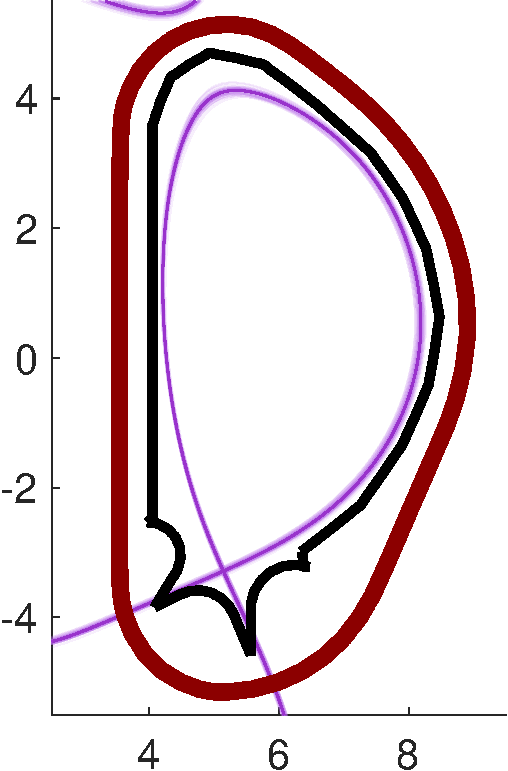
\includegraphics[width=0.19\linewidth]{./figures/QoI_MC_uniform.pdf}
% &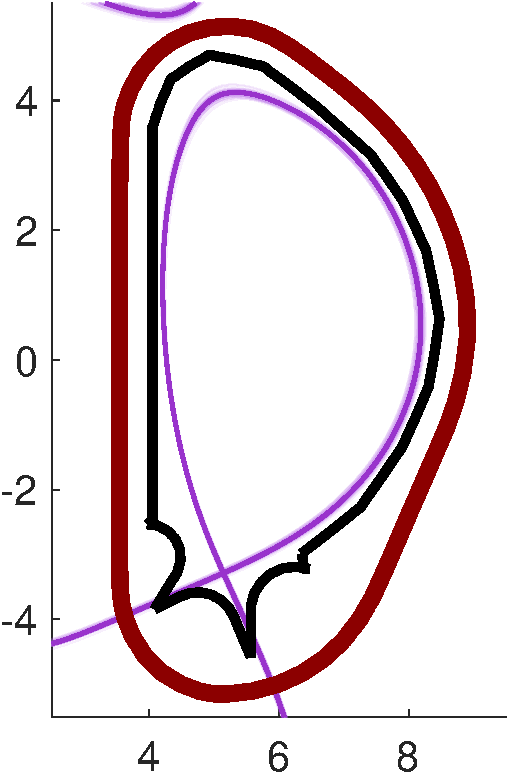
\includegraphics[width=0.19\linewidth]{./figures/QoI_MC_surrogate.pdf}
&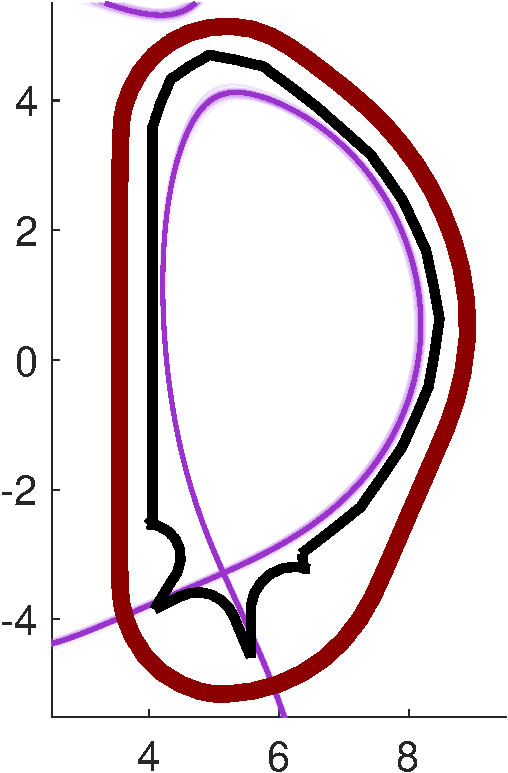
\includegraphics[width=0.19\linewidth]{./figures/QoI_MLMC_DirectSolver_Interp2CommonGrid.pdf} 
& 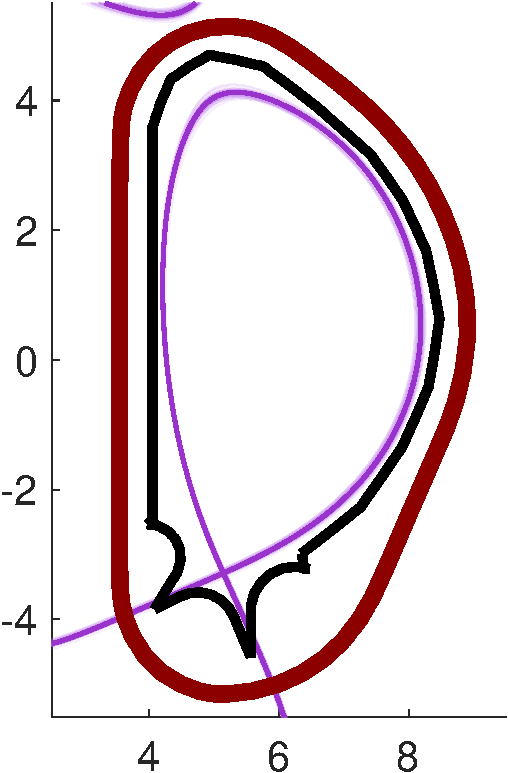
\includegraphics[width=0.19\linewidth]{./figures/QoI_MFMC.pdf} 
\\
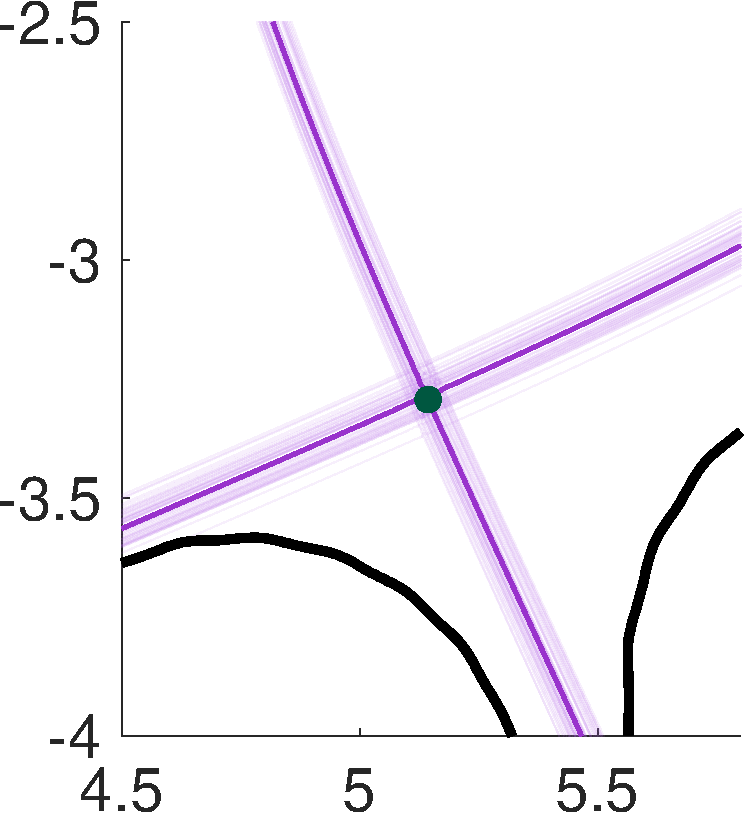
\includegraphics[width=0.19\linewidth]{./figures/QoI_MC_uniform_xptRegion.pdf} 
% &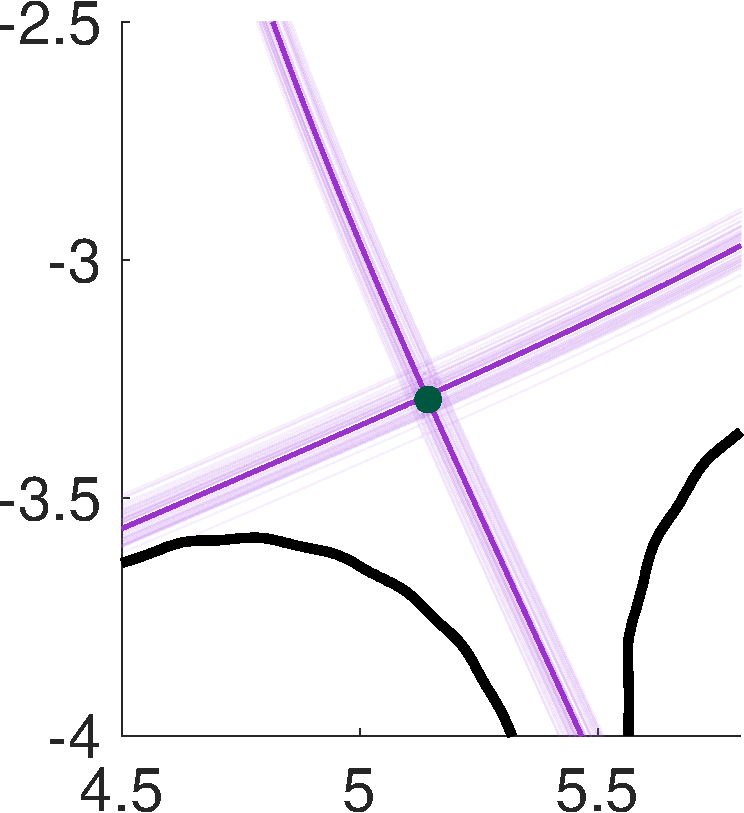
\includegraphics[width=0.19\linewidth]{./figures/QoI_MC_surrogate_xptRegion.pdf}
&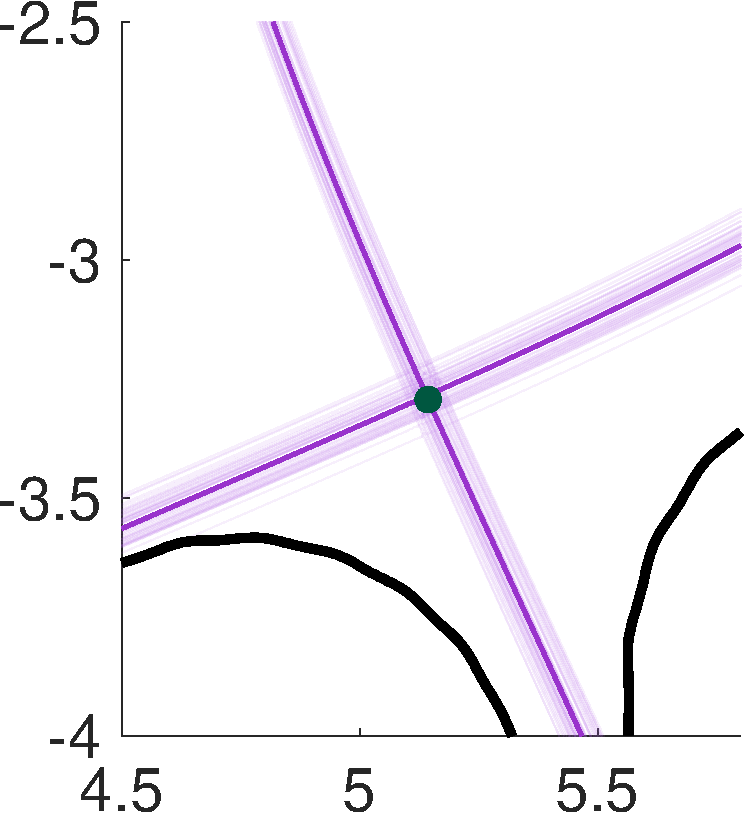
\includegraphics[width=0.19\linewidth]{./figures/QoI_MLMC_DirectSolver_xptRegion_Interp2CommonGrid.pdf} 
&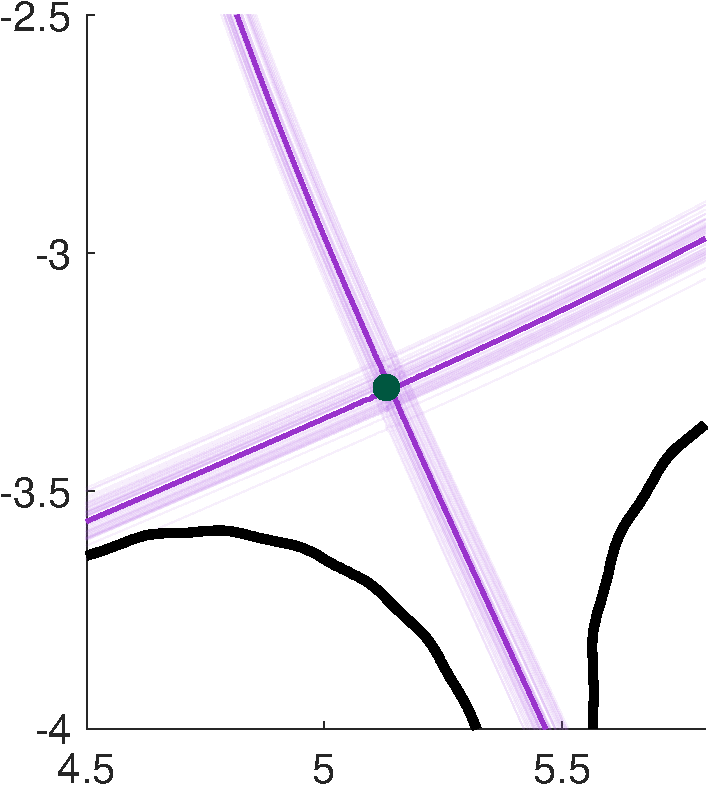
\includegraphics[width=0.19\linewidth]{./figures/QoI_MFMC_xptRegion.pdf} 
\\[1ex]
\quad MC-FE &MLMC-FE (Interp) &MFMC-FE (Interp) \\[-0.5ex]
\end{tabular}
\caption{The plasma boundaries of 50 random realizations are overlaid in the top row as violet curves. The solid violet line represents the plasma boundary of the expected poloidal flux generated with tolerance $\epsilon=4\times 10^{-4}$. The reactor's inner and outer walls are shown in solid black and dark red, respectively. The bottom row provides a detailed view of the regions close to the x-points, with dark green dots indicating the x-points of the expected solution. The columns, from left to right, show the simulations using the MC-FE, MLMC-FE, and MFMC-FE approaches, all interpolated to geometry-conforming uniform meshes at discretization level $\ell=5$.}
\label{fig:QoI_plot}
\end{figure}
%














% \noindent \textbf{Geometric descriptors.}
%
\begin{table}[ht]
	\centering
			\scalebox{0.6}{
		\begin{tabular}{c|c|c|c|c|c|c|}
			\cline{2-5}
				&\multicolumn{1}{c|}{MC-FE}&MLMC-FE&MLMC-FE (Interp)&MFMC-FE (Interp)\\
			\hline
			\multicolumn{1}{|c|}{x point}&(5.14,-3.29)&(5.14,-3.29)&(5.14,-3.29)&(5.14,-3.29)\\
			\hline
			\multicolumn{1}{|c|}{magnetic axis}&(6.41,0.61)&(6.44,0.56)&(6.41,0.61)&(6.41,0.61)\\
			\hline
			\multicolumn{1}{|c|}{strike} &(4.16,-3.71)&(4.16,-3.71)&(4.16,-3.71)&(4.16,-3.71)\\
			\multicolumn{1}{|c|}{points}&(5.56,-4.22)&(5.56,-4.22)&(5.56,-4.22)&(5.56,-4.22)\\
			\hline
			\multicolumn{1}{|c|}{inverse aspect ratio} &0.32&0.32&0.32&0.32\\
			\hline
			\multicolumn{1}{|c|}{elongation} &1.86&1.87&1.86&1.86\\
			\hline
			\multicolumn{1}{|c|}{upper triangularity}&0.43&0.43&0.43&0.43\\
			\hline
			\multicolumn{1}{|c|}{lower triangularity} &0.53&0.53&0.53&0.53\\
			\hline
	\end{tabular}
  }
	\caption{Geometric parameters of the expected poloidal flux $u$ for different simulation methods: MC-FE with direct solver, MLMC-FE with direct solver, MLMC-FE with direct solver and interpolation of the solution to a common fine grid at level $\ell=5$, and MFMC-FE with interpolation of the solution to a common fine grid at level $\ell=5$. The results are generated with an nMSE of $4 \times 10^{-4}$.}
	\label{Tab:QoI_GeoInfo}
\end{table}







% % =============================
% \subsection{Uncertainties in the source term}
% % =============================
% In this experiment, we study the uncertainty in perturbing the reference parameter that characterizes the source term \eqref{eq:source}.
% \begin{table}[ht]
% 	\centering
% 			\scalebox{0.62}{
%    \begin{tabular}{c|c|c|c|c|c|c|c|c|c|c|c|c|}
% 	    \cline{2-7}	
% 		&\multicolumn{6}{|c|}{ Level $\ell$}\\
% 			\hline
% 			\multicolumn{1}{|c|}{$\epsilon$}&0&1&2&3&4&5\\
% 			\hline
% 			\multicolumn{1}{|c|}{$8\times 10^{-3} $}&&&8&&&\\
% 			\multicolumn{1}{|c|}{$6\times 10^{-3} $}&&&10&&&\\
% 			\multicolumn{1}{|c|}{$4\times 10^{-3} $}&&&&25&&\\
% 			\multicolumn{1}{|c|}{$2\times 10^{-3} $}&&&&93&&\\
% 			\multicolumn{1}{|c|}{$10^{-3} $}&&&&&423&\\
% 			\multicolumn{1}{|c|}{$8\times 10^{-4} $}&&&&&678&\\
% 			\multicolumn{1}{|c|}{$6\times 10^{-4} $}&&&&&1211&\\
%                 \multicolumn{1}{|c|}{$4\times 10^{-4} $}&&&&&2700$^{\ast}$&\\
%                 \multicolumn{1}{|c|}{$2\times 10^{-4} $}&&&&&&11000$^{\ast}$\!\!\\
% 			\hline
% 	\end{tabular}
%  \qquad
% 		\begin{tabular}{c|c|c|c|c|c|c|c|c|c|c|c|c|}
% 	    \cline{2-7}	
% 		&\multicolumn{6}{|c|}{ Level $\ell$}\\
% 			\hline
% 			\multicolumn{1}{|c|}{$\epsilon$}&0&1&2&3&4&5\\
% 			\hline
% 			\multicolumn{1}{|c|}{$8\times 10^{-3} $}&10 &2 &2&&&\\
% 			\multicolumn{1}{|c|}{$6\times 10^{-3} $}&11 &3 &2 &&&\\
% 			\multicolumn{1}{|c|}{$4\times 10^{-3} $}&33 &7 &2 &2&&\\
% 			\multicolumn{1}{|c|}{$2\times 10^{-3} $}&150 &27 &4 &2&&\\
% 			\multicolumn{1}{|c|}{$10^{-3} $}&692 &116 &19 &4 &2&\\
% 			\multicolumn{1}{|c|}{$8\times 10^{-4} $}&1008 &160 &27 &6 &2&\\
% 			\multicolumn{1}{|c|}{$6\times 10^{-4} $}&2022 &322 &53 &10 &3&\\
%                 \multicolumn{1}{|c|}{$4\times 10^{-4} $}&4158 &613 &106 &14 &4&\\
%                 \multicolumn{1}{|c|}{$2\times 10^{-4} $}&17158 &2612 &442 &59 &13 &2\\
% 			\hline
% 	\end{tabular}
%  \qquad
% 		\begin{tabular}{c|c|c|c|c|c|c|c|c|c|c|c|c|c|c|c|c|c|}
% 	    \cline{2-7}	
% 		&\multicolumn{6}{|c|}{ Level $\ell$}\\
% 			\hline
% 			\multicolumn{1}{|c|}{$\epsilon$}&0&1&2&3&4&5\\
% 			\hline
% 			\multicolumn{1}{|c|}{$8\times 10^{-3} $}&&&&&&\\
% 			\multicolumn{1}{|c|}{$6\times 10^{-3} $}&&&&&&\\
% 			\multicolumn{1}{|c|}{$4\times 10^{-3} $}&&&\\
% 			\multicolumn{1}{|c|}{$2\times 10^{-3} $}&&&\\
% 			\multicolumn{1}{|c|}{$10^{-3} $}&&&&&&\\
% 			\multicolumn{1}{|c|}{$8\times 10^{-4} $}&&&&&&\\
%                 \multicolumn{1}{|c|}{$6\times 10^{-4} $}&&&&&&\\
% 			\multicolumn{1}{|c|}{$4\times 10^{-4} $}&&&&&&\\
%                 \multicolumn{1}{|c|}{$2\times 10^{-4} $}&&&&&&\\
% 			\hline
% 	\end{tabular}
 
%  }
% 	\caption{The optimal sample size estimation for MC-FE (left), uniform MLMC-FE (middle), and MFMC-FE (right). The simulations were conducted for a variety of choices of $\epsilon$. The computational cost associated with a tolerance of $\epsilon = 2\times 10^{-4}$ for Monte Carlo was prohibitive; the entry in the table for this tolerance (with an asterisk) is an estimate.}
% 	\label{Tab:SampleSize_Source_Term}
% \end{table}

% \begin{table}[ht]
% 	\centering
% 			\scalebox{0.62}{
%    \begin{tabular}{c|c|c|c|c|c|c|c|c|c|c|c|c|}
% 			\hline
% 			\multicolumn{1}{|c|}{ }&MC-FE &MLMC-FE &MFMC-FE\\
% 			\multicolumn{1}{|c|}{$\epsilon$}&Time & \begin{tabular}{cc} \,\,\,\,\,Time & \,\,\,Speedup \end{tabular}  &\begin{tabular}{cc} \,\,\,\,Time & \,\,\,Speedup \end{tabular}\\
% 			\hline
% 			\multicolumn{1}{|c|}{$8\times 10^{-3} $}&9.71e+01&\begin{tabular}{cc}1.10e+01\,\,\, & 8.8 \end{tabular}&\begin{tabular}{cc}..\,\,  & .. \end{tabular} \\
% 			\multicolumn{1}{|c|}{$6\times 10^{-3} $}&1.16e+02&\begin{tabular}{cc}1.27e+01\,\,\, & 9.1 \end{tabular}&\begin{tabular}{cc}..\,\, &.. \end{tabular}\\
% 			\multicolumn{1}{|c|}{$4\times 10^{-3} $}&1.29e+02&\begin{tabular}{cc}3.39e+01\,\,\, & 3.8 \end{tabular}&\begin{tabular}{cc}..& .. \end{tabular}\\
% 			\multicolumn{1}{|c|}{$2\times 10^{-3} $}&8.03e+02&\begin{tabular}{cc}7.29e+01\,\, & 11.0\end{tabular}&\begin{tabular}{cc}..& .. \end{tabular}\\
% 			\multicolumn{1}{|c|}{$10^{-3} $}&1.49e+04&\begin{tabular}{cr}2.55e+02\,\, & 58.5 \end{tabular}&\begin{tabular}{cc}..& .. \end{tabular}\\
% 			\multicolumn{1}{|c|}{$8\times 10^{-4} $}&3.89e+04&\begin{tabular}{cc}2.76e+02\,\, &140.6 \end{tabular}&\begin{tabular}{cc}..& ..
%             \end{tabular}\\
% 			\multicolumn{1}{|c|}{$6\times 10^{-4} $}&1.1219e+05&\begin{tabular}{cc}7.1946e+02\,\, & .. \end{tabular}&\begin{tabular}{cc}.. & .. \end{tabular}\\
%                 \multicolumn{1}{|c|}{$4\times 10^{-4} $}&..&\begin{tabular}{cc}1.1598e+03\,\, & .. \end{tabular} &\begin{tabular}{cc}..& .. \end{tabular}\\
%                 \multicolumn{1}{|c|}{$2\times 10^{-4} $}&..$^{\ast}$\!\!\!&\begin{tabular}{cc}4.4956e+03 &.. \end{tabular} &\begin{tabular}{cc}..&.. \end{tabular}\\
% 			\hline
% 	\end{tabular}
%  }
% 	\caption{The CPU time in seconds for MC-FE (left), uniform MLMC-FE (middle), and MFMC-FE (right), together with speedups for the multilevel methods, for a variety of choices of $\epsilon$. The computational cost associated with a tolerance of $\epsilon = 2\times 10^{-4}$ for Monte Carlo was prohibitive; the entry in the table for this tolerance (with an asterisk) is an estimate.}
% 	\label{Tab:CPU_time_Source_Term}
% \end{table}